\documentclass[letterpaper, 11pt]{article}


%=================================================

\usepackage{fullpage, parskip}
\usepackage{fancyhdr}
\usepackage{amsmath, mathtools,amssymb}
\usepackage{graphicx}
\usepackage{tabularx}
\usepackage{xspace}
\usepackage{natbib}
%% Journal control sequences
\usepackage{aas_macros} 

%--------------------------------------------------
\def\humvi{{\sc HumVI}\xspace}

%--------------------------------------------------
%% Header and Footer
\pagestyle{fancy}
\fancyhead{}
\renewcommand{\headrulewidth}{0.0pt}
\rfoot{HumVI}
\lfoot{December 2012}

%% Top matter
\title{HumVI: Image Stretching and Scaling Tests}
\author{Phil Marshall\thanks{\texttt{dr.phil.marshall@gmail.com}}, 
Cato Sandford, David Hogg, Amit Kapadia}
\date{\today}

%%-------------------------------------------------

\begin{document}

\maketitle
\vspace{1cm}


\begin{abstract}
We investigate some useful input parameters for
use when composing color images from the data in the CFHTLS.
\end{abstract}


\section{Introduction}
\label{sec:intro}

Suppose we have a large set of imaging data from a given sky survey. We would
like to make color representations of the images in this set, such that they
can be a) compared with each other, to build intuition about the data quality
and the appearance of objects in the survey, and b) searched for low surface
brightness, color-contrasting features. We use the \humvi python
implementation of the \citet[][hereafter L04]{Lup++04} algorithm, with some simplifications and
extensions. For simplicity we use a single filter for each RGB channel,
choosing the {\it i}, {\it r} and {\it g} bands respectively.

\section{Scaling and Stretching the Images}
\label{sec:stretch}

The scaling and stretching of the input images is controlled by three
parameters. The three \texttt{scales} parameters, one for each channel, are
used to multiply the channel images before any other operations are performed.
The \texttt{scales} account for any difference in units between the images,
and also the sensitivity of the detector in that filter, the exposure time
used, and so on. We denote this scale parameter by $s_{X}$ where $X$ is one of
the channel identifiers, $R,G,B$. For convenience, we normalize the scales to
have unit mean, since it will often be the case that the images taken in
different filters will have the same units and approximately equal pixel
values. Crucially, these scales can be chosen to be the same for all images in
a survey, allowing different images to be compared with each other; likewise
they can be used to account for variations in, for example, exposure time
between images.

After scaling, the total intensity image is
computed, and used to compute the stretch factor, which is governed by two
parameters, $Q$ and $\alpha$ as given by L04:
\begin{align}
I &= r s_R + g s_G + b s_B \\
X(I) &= \frac{1}{QI}\cdot{\rm arcsinh}(\alpha Q I) \\
R &= r s_R X \\
G &= g s_G X \\
B &= b s_B X \\
\end{align}
For small values of $\alpha Q I$, $X \approx \alpha$, and constant: at low
intensity, each channel image is simply rescaled by $\alpha$. Low surface
brightness features are made more visible by increasing $\alpha$. 
At higher values, 
the arcsinh function reduces this scale factor, making high intensity regions
less saturated. The onset of this behavior occurs when $\alpha Q I \approx 1$,
or when $I \approx 1 / \alpha Q$. 
In order to make a PNG image, \humvi works to make three channel images whose
values are clipped at zero and one. This choice of 1 as the maximum pixel
value allows us to choose $Q$ and $\alpha$ sensibly. For example, suppose we
have a set of scaled images with approximately zero mean, unit 
rms and brightest pixel
value $10^4$. If we want a pixel with value 3 times the rms to have
normalized value 0.1 in each channel of 
the final image, then we need $X(9)=1/30$ ($I\approx9$ if each channel image
pixel value is about $3-\sigma$). We'd
like this to still be in the linear regime, so we need $9 \alpha Q \ll 1$,
and also $\alpha \approx 1/30 \approx 0.03$. Combining these two requirements,
we find that we need $Q
\ll 3$. The algorithm is not very sensitive to the value of $Q$, as long as
it is very much less than $1/\alpha$. 
Drawing a parallel with television controls,
$Q$ behaves like the brightness, while $\alpha$ is like the contrast.

In Figure~\ref{fig:stretch} we show, for a fixed set of scales, the effect of
varying $\alpha$ and $Q$ when displaying an image that has approximately unit
rms pixel value in each channel. The values $\alpha = 0.03$ and $Q = 1$
provide a good representation of the image. 

\begin{figure}
\centering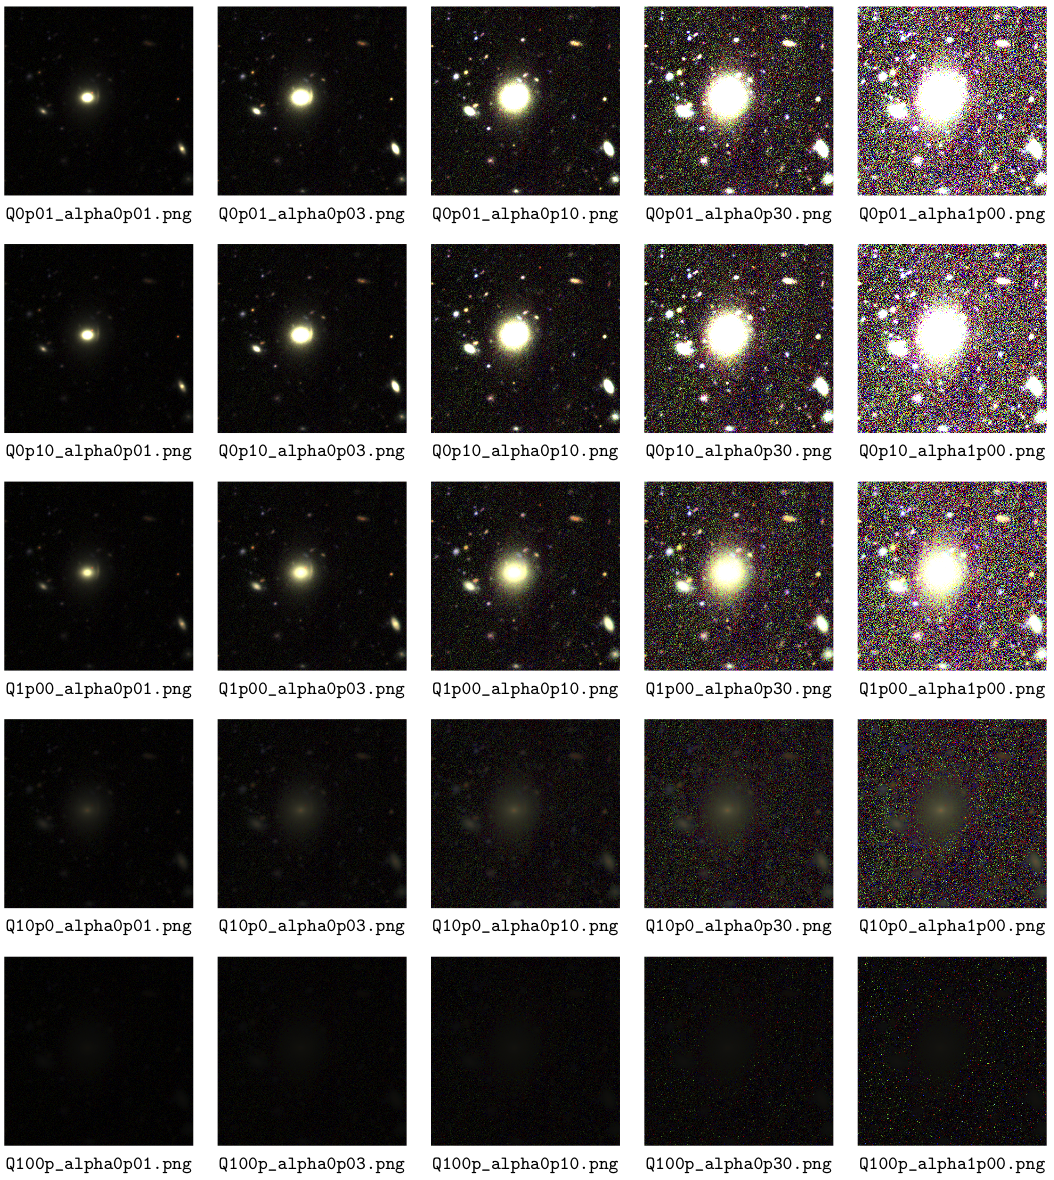
\includegraphics[width=0.9\linewidth]{Images/CFHTLS_27_Q-alpha_gallery.png}
\caption{The effect of the non-linearity parameters $Q$ and $\alpha$ on an
example image from the CFHTLS survey. Left to right, $\alpha$ increases
through the set $\{0.01,0.03,0.1,0.3,1.0\}$. Top to bottom, $Q$ increases
through the set $\{0.01,0.1,1.0,10,100\}$.}
\label{fig:stretch}
\end{figure}

\section{Saturation and Thresholding}
\label{sec:saturation}

The scaled and stretched pixel values of the previous section have to be
mapped onto a unit range for encoding in a PNG image. How we deal with pixels
that fall outside that range will affect the appearance of the composite.

At low brightness, we have to decide which pixels we want to appear black.
Background-subtracted images will have negative pixel values in the ``blank''
sky regions. One option is to set all pixels with value less than zero to
zero. This leads to a large number of black pixels (approximately half of
them!) and a strong impression of dark sky. If we want to retain the
information that those negative pixels contain (about the noise level), we can
add an offset $\delta$ to each scaled and stretched channel image, such that
pixels with value $-delta$ appear black in the final composite. This has the
effect of making the blank regions of the image appear dark gray instead of
black. Choosing $\delta$ to be negative has the opposite effect, making the
sky look blacker than black... Figure~\ref{fig:offset} shows the effect of
various offset values on the appearance of the test image from
Figure~\ref{fig:scaling}. We find that actually an offset of zero is a good
compromise between ``seeing the noise'' and achieving a nice dark background
against which low surface brightness features can be seen.

\begin{figure}
\centering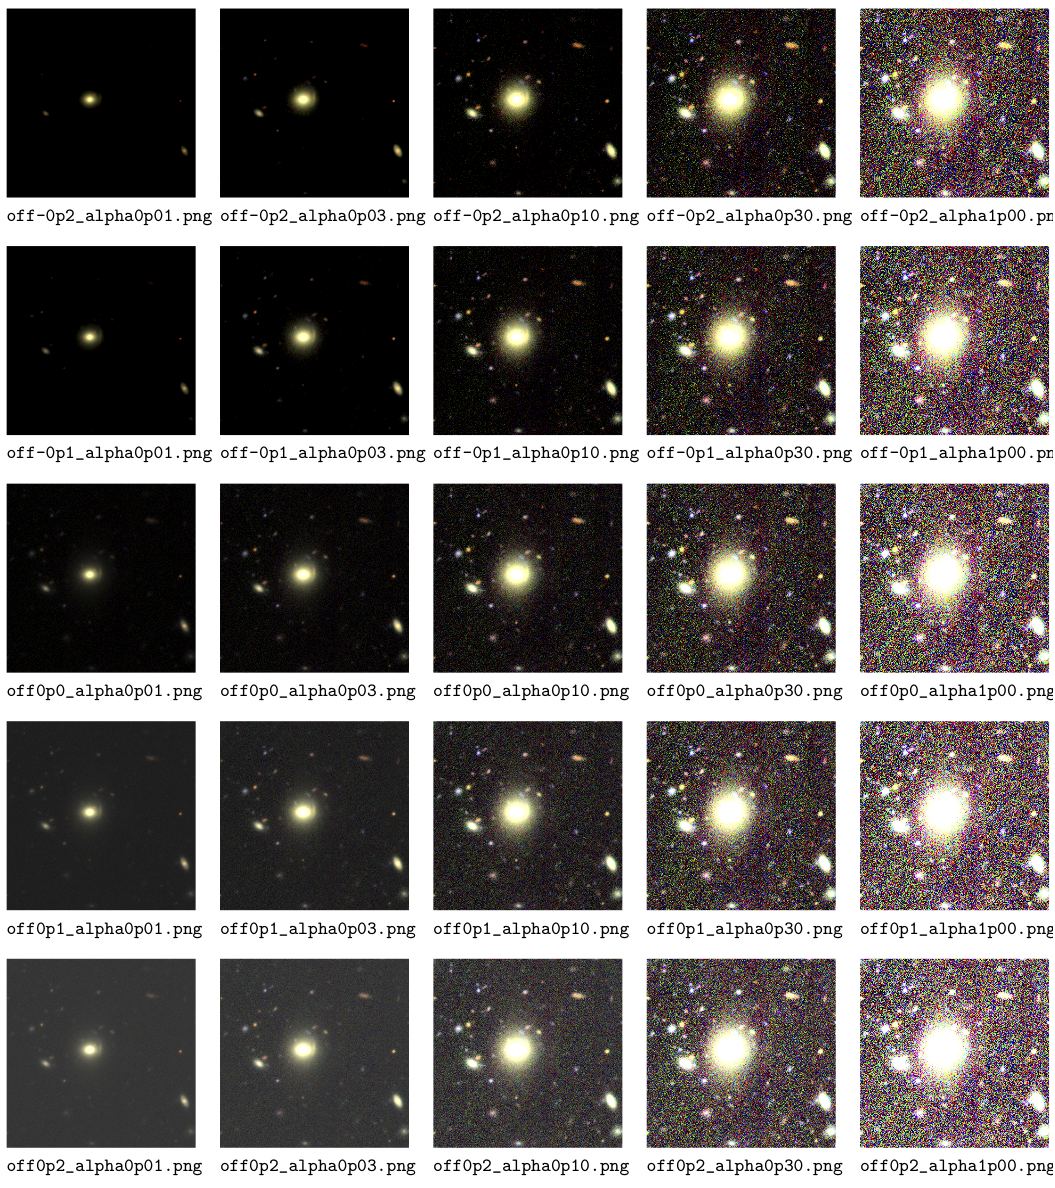
\includegraphics[width=0.9\linewidth]{Images/CFHTLS_27_offset-alpha_gallery.png}
\caption{The effect of the offset parameter $\delta$ and contrast 
$\alpha$ on an
example image from the CFHTLS survey. Left to right, $\alpha$ increases
through the set $\{0.01,0.03,0.1,0.3,1.0\}$. Top to bottom, $\delta$ increases
through the set $\{-0.2,-0.1,0.0,0.1,0.2\}$.}
\label{fig:offset}
\end{figure}

At the bright end we have a different choice to make: what to do in pixels
whose values are greater than 1 in any channel? In Figures~\ref{fig:stretch}
and~\ref{fig:offset} we simply snapped thes pixel values to one in that
channel, a procedure that leads to ``saturation to white'' in the case where
all three channel pixel values exceed 1. An alternative is to snap the highest
pixel value of an RGB triplet to 1, and then rescale the other two so as to
preserve the {\it color} of the pixel. This was advocated in L04. The two
approaches are shown in Figure~\ref{fig:saturation}, again as a function of
$\alpha$. If the image is not stretched too hard, saturation to white is not
an issue, as all pixels remain in the required 0:1 range. Note that the faint
objects in the low $\alpha$ frames in Figure~\ref{fig:saturation} look very
similar between the two saturation schemes. With
color-preserving saturation we see some odd effects: red central cores and
ring-like artifacts which, while providing more information about the images,
may provide distractions during a search for low surface brightness features. 
The contrasting (eg yellow) rings around faint (eg red) objects is likely to
be a result of PSF mismatch between these images: if the resolutions of the
three channels' images are not well-matched, confusing artifcacts will arise.
Saturation to white seems to be an {\it easy way to hide this problem}.

\begin{figure}
\centering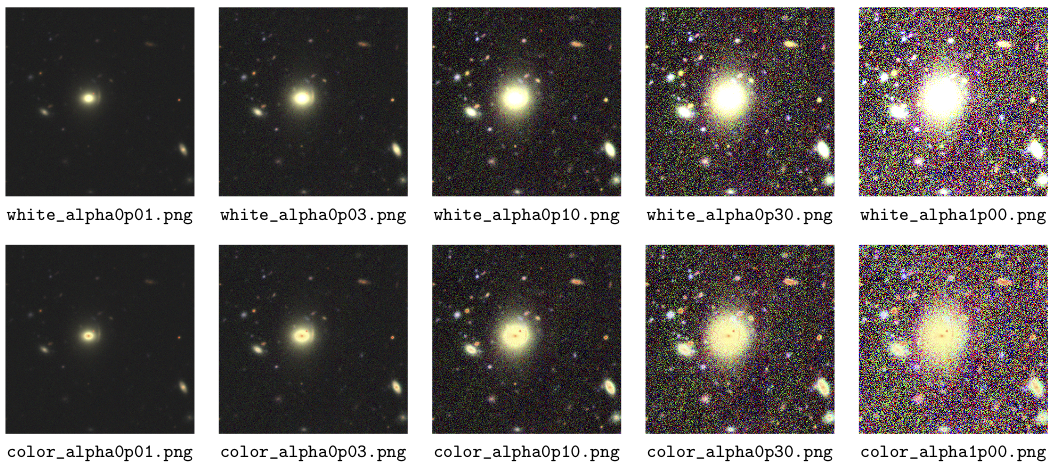
\includegraphics[width=0.9\linewidth]{Images/CFHTLS_27_saturation_gallery.png}
\caption{The effect of the saturation scheme on an
example image from the CFHTLS survey. Left to right, $\alpha$ increases
through the set $\{0.01,0.03,0.1,0.3,1.0\}$. Top row: saturation to white;
Bottom row: color-preserving saturation, as proposed by L04.}
\label{fig:saturation}
\end{figure}


\section{Color Balance}
\label{sec:color}

Finally, we return to the choice of scales for a composite image, which is
best made after setting the stretch and saturation parameters well. The
scales should reflect the quality of each channel's image, including
the sensitivity of the instrumentation, the filter transmission, the exposure
time and so on. However, the relative scales can also be chosen to change the
balance of color in the image, in order to improve the color contrast between
different objects. In Figure~\ref{fig:color} we show the effect of varying the
scales by small amounts around their natural (unit) values.

A good strategy when looking for contrasting features around massive galaxies
could be to choose scales such that the massive galaxies appear as bright
yellow as possible, and the objects around them as different as possible. The
set $\{0.8,1.0,1.0\}$ seems to work reasonably well in this example.

\begin{figure}
\centering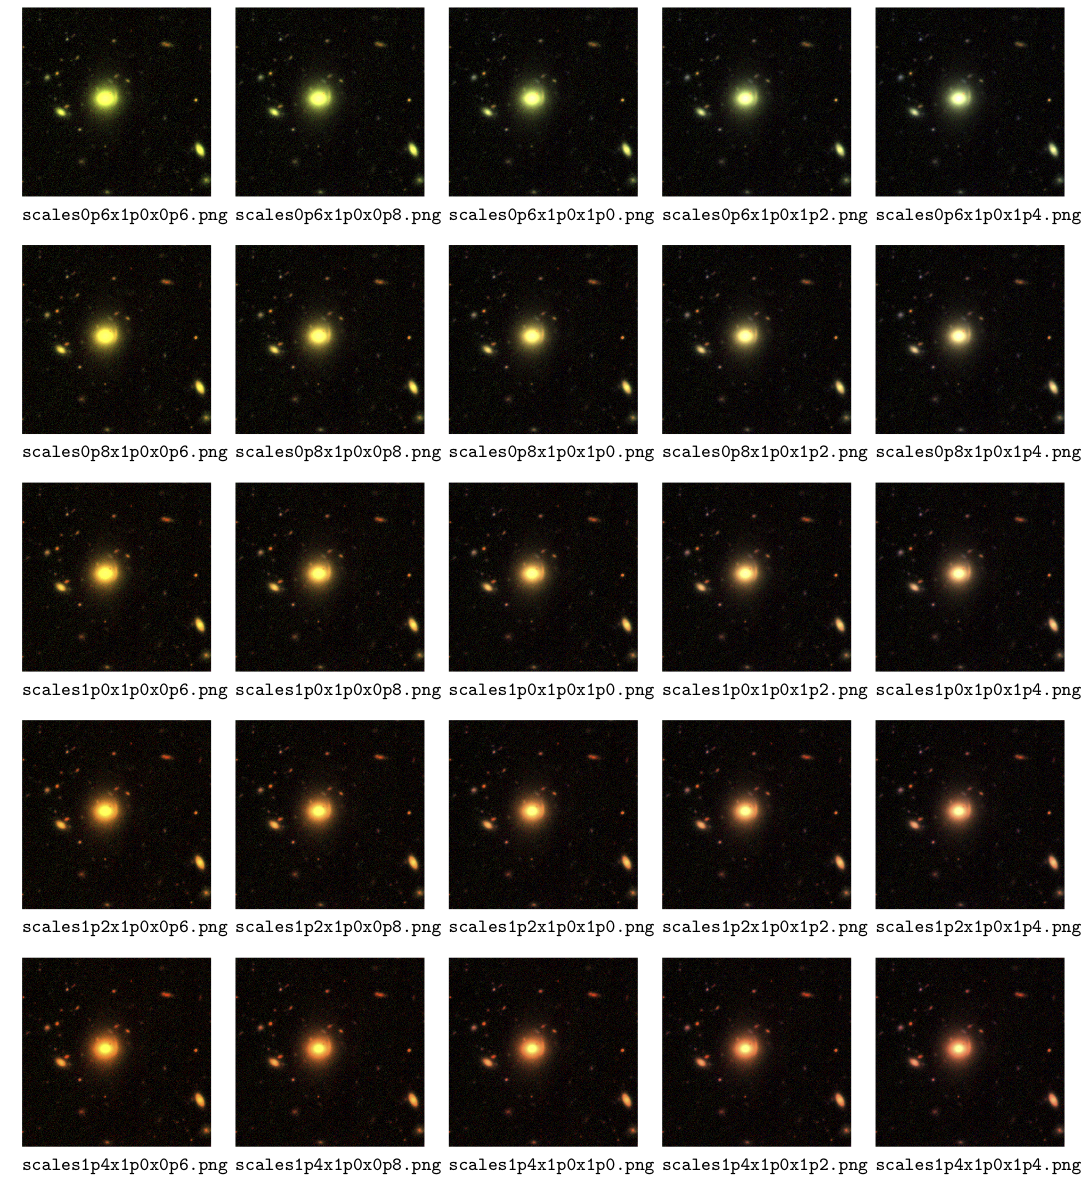
\includegraphics[width=0.9\linewidth]{Images/CFHTLS_27_scales_gallery.png}
\caption{The effect of changing the relative image scales on the color balance
in an example image from the CFHTLS survey. We keep the G channel image scale
fixed at 1.0. Left to right, the R channel image scale increases through the
set $\{0.6,0.8,1.0,1.2,1.4\}$. Top to bottom, the B channel image increases
through the same set. $Q=1.0$ and $\alpha = 0.03$.}
\label{fig:color}
\end{figure}


\section{Conclusions}
\label{sec:color}

From these explorations we conclude:
\begin{itemize}
\item $\alpha$ is the key ``contrast'' parameter needed to bring out low
surface brightness features in an image.
\item If all images in a set were taken under the same conditions, only the
relative scales need be specified.
\item These relative scales determine the color balance of the image, and
should be chosen by experimentation.
\item The $Q$ parameter is a ``brightness'' control, and has less effect on an
image than $\alpha$; however, they do need to be set together.
\item Future work using images with varying conditions may need unnormalized
scales, in which case $Q$ may become somewhat, although not completely, 
redundant.
\item While color-preserving saturation retains more information in the image,
this information may be distracting during a low surface brightness feature
search.
\item Matching the resolutions of the input channel images may mitigate
against some of the artifacts highlighted by the saturate to color algorithm.
\end{itemize}


\section{References}

\bibliographystyle{mn2e}
\bibliography{humvi}

\end{document}
